\chapter{图上的神经网络}
\label{chap:graph-neural-networks}
\begin{quote}\small
\textit{本章摘要。}本章研究怎样把设备之间的连接和多个设备共同参与的关系用于预测。从图数据、节点定义与预测对象开始，先区分设备、变量、时间步和变量--时间片等建图单位，再建立消息传递的计算框架。随后展开图卷积网络的节点更新、归一化、手算例子及谱滤波来源，固定聚合系数的局限引出邻域采样和图注意力。最后用关联矩阵表示超图，推导节点到超边再返回节点的超图卷积，说明线性传播与成对图传播的联系，并讨论表示退化、信息压缩、建图边界与工业验证。
\end{quote}

前面的序列模型利用时间顺序，视觉模型利用像素的空间邻域。设备系统还包含另一类结构：设备通过管路、电路或生产流程相连。预测某台泵的状态时，它自己的振动记录可能不足，还需要读取上游设备的运行状态。这里的邻近由连接关系决定，设备编号相邻不表示设备相连。

考虑一个教学任务：在每个预测时刻，利用当前可用的运行记录，预测每台设备未来二十四小时内是否发生故障。序列编码器可以先把每台设备此前的读数变成特征，图模型再交换相关设备的信息。输入仍受预测时刻限制，设备连接也必须在该时刻已知。事后确认的故障传播路径不能直接用于此前的预测。

本章先回答一条边如何改变节点计算，再回答多个节点共同参与的关系怎样进入网络。理解主要公式需要矩阵乘法、非线性函数与分类损失。谱滤波小节还用到实对称矩阵的特征分解，可在完成节点手算后阅读。

\section{图表示与预测对象}
\subsection{节点、边与节点特征}
图（graph）记为$G=(\mathcal V,\mathcal E)$，其中$\mathcal V$是节点集合，$\mathcal E$是边集合。设有$n$个节点。节点是一次建模选定的基本单位，可以是一台设备、一只传感器、一个工序、一个测量变量、一个时间步或一个变量的时间片。物理传感器与测量变量未必一一对应：一台设备可以带有多只传感器，一只三轴振动传感器也可以产生三个测量通道。一次建模应明确节点对应的对象，不能在没有说明的情况下混用这些含义。边表示允许交换信息的关系，例如管路连接、工艺上的直接依赖或任务允许的时间联系。

用邻接矩阵$A\in\R^{n\times n}$记录连接。本章按$A_{ij}$表示节点$j$向节点$i$提供信息，因此$(AX)_i=\sum_j A_{ij}X_j$读取的是节点$i$的输入邻居。无权图中，相连时$A_{ij}=1$，否则为零。除专门讨论有向图的段落外，以下GCN与谱推导假设$A=A^{\mathsf T}$、$A_{ij}\geq0$，原图无自环。记$\mathcal N(i)=\{j\ne i:A_{ij}>0\}$为邻居集合。

每个节点的初始特征为列向量$\bm x_i\in\R^d$，将其转置后按行排列：
\begin{equation}
 X=\begin{bmatrix}\bm x_1^{\mathsf T}\\\vdots\\\bm x_n^{\mathsf T}\end{bmatrix}\in\R^{n\times d},\qquad H^{(0)}=X.
 \label{eq:graph-feature-matrix}
\end{equation}
一般情况下，$n$是节点数，$d$是每个节点的特征维数。隐藏层特征矩阵$H^{(\ell)}\in\R^{n\times d_\ell}$的第$i$行记为$\bm h_i^{(\ell)\mathsf T}$，保持本书向量默认为列向量的约定。本章后续以设备图为主要例子时，节点才对应设备。例如，设备的温度、振动和负载经过训练集确定的标准化后可形成三维输入。不同物理单位的原始数值不宜未经处理就比较大小。

同一批工业观测可以按不同单位建图，表\ref{tab:graph-node-units}列出四种常见选择。以变量为节点时，图关系可以来自机理先验，也可以由训练数据学习。例如MTGNN用图学习模块刻画多变量时间序列中的变量关系\footnote{来源：Wu等，\href{https://arxiv.org/abs/2005.11650}{\textit{Connecting the Dots: Multivariate Time Series Forecasting with Graph Neural Networks}}，2020。}。学习到的统计边不自动等同于真实物理连接或因果关系。

\begin{table}[htbp]
\centering
\caption{不同建图单位中的节点、特征与边}
\label{tab:graph-node-units}
\footnotesize
\setlength{\tabcolsep}{2.5pt}
\renewcommand{\arraystretch}{1.18}
\begin{tabular}{@{}>{\raggedright\arraybackslash}m{0.11\linewidth}>{\raggedright\arraybackslash}m{0.17\linewidth}>{\raggedright\arraybackslash}m{0.20\linewidth}>{\raggedright\arraybackslash}m{0.18\linewidth}>{\raggedright\arraybackslash}m{0.20\linewidth}@{}}
\toprule
建图单位 & 节点代表什么 & 节点特征 & 边可以表示什么 & 需要保留的边界 \\
\midrule
设备 & 一台泵、电机或其他设备 & 该设备多变量历史的摘要或序列编码 & 管路、电路或工序依赖 & 一台设备可带多只传感器和多个测量通道 \\
变量 & 温度、转速、振动幅值等一个测量通道 & 该变量的一段历史或其表示 & 机理联系、统计依赖或学习关系 & 三轴传感器可产生多个变量。统计边不等于因果边 \\
时间步 & 历史窗口内的一个时刻 & 该时刻的多变量观测 & 相邻时间、给定时滞或任务允许的历史联系 & 特征与连接均受预测时刻的信息边界约束 \\
变量--时间片 & 某个变量的一段连续历史 & 该时间片的数值或嵌入 & 同变量跨片、异变量同片位或跨片位关系 & 节点数同时随变量数和时间片数变化 \\
\bottomrule
\end{tabular}
\end{table}

图\ref{fig:graph-node-units}把同一类设备、变量和历史观测画成四种具体节点，其中$T$、$v$、$\omega$、$I$分别表示温度、振动、转速和电流。各栏中的线段或箭头只说明该建图下允许的信息联系，不能把设备连接直接解释成变量因果关系，也不能把时间边自动套到设备图上。

\begin{figure}[htbp]
\centering
\begin{tikzpicture}[x=1cm,y=1cm]
 \draw[rounded corners=3pt,gray!60] (-0.2,-0.2) rectangle (6.2,2.7);
 \node[font=\small\bfseries] at (3,2.42) {设备节点};
 \node[idi input,minimum width=2.15cm,minimum height=0.65cm,inner sep=3pt,font=\scriptsize] (dev-a) at (1.45,1.25) {泵A\\特征：$T,v$};
 \node[idi input,minimum width=2.15cm,minimum height=0.65cm,inner sep=3pt,font=\scriptsize] (dev-b) at (4.75,1.25) {电机B\\特征：$\omega,I$};
 \draw[thick] (dev-a)--node[above,font=\scriptsize]{传动连接}(dev-b);
 \node[font=\scriptsize,align=center] at (3,0.35) {节点是物理设备。一台设备可含多个变量};

 \draw[rounded corners=3pt,gray!60] (6.6,-0.2) rectangle (13,2.7);
 \node[font=\small\bfseries] at (9.8,2.42) {变量节点};
 \node[idi input,minimum width=1.55cm,minimum height=0.65cm,inner sep=3pt,font=\scriptsize] (var-t) at (7.7,1.25) {温度$T$\\历史窗口};
 \node[idi input,minimum width=1.55cm,minimum height=0.65cm,inner sep=3pt,font=\scriptsize] (var-v) at (9.8,1.25) {振动$v$\\历史窗口};
 \node[idi input,minimum width=1.55cm,minimum height=0.65cm,inner sep=3pt,font=\scriptsize] (var-w) at (11.9,1.25) {转速$\omega$\\历史窗口};
 \draw[thick] (var-t)--(var-v); \draw[thick] (var-v)--(var-w);
 \node[font=\scriptsize,align=center] at (9.8,0.35) {边：机理联系、统计依赖或学习关系};

 \draw[rounded corners=3pt,gray!60] (-0.2,-3.65) rectangle (6.2,-0.55);
 \node[font=\small\bfseries] at (3,-0.85) {时间步节点};
 \node[idi state,minimum width=1.35cm,minimum height=0.65cm,inner sep=3pt,font=\scriptsize] (time-a) at (1.05,-2.05) {$t-2$\\$[T,v]$};
 \node[idi state,minimum width=1.35cm,minimum height=0.65cm,inner sep=3pt,font=\scriptsize] (time-b) at (3,-2.05) {$t-1$\\$[T,v]$};
 \node[idi state,minimum width=1.35cm,minimum height=0.65cm,inner sep=3pt,font=\scriptsize] (time-c) at (4.95,-2.05) {$t$\\$[T,v]$};
 \draw[idi arrow] (time-a)--(time-b); \draw[idi arrow] (time-b)--(time-c);
 \node[font=\scriptsize,align=center] at (3,-3.1) {节点特征是同一时刻的多变量观测};

 \draw[rounded corners=3pt,gray!60] (6.6,-3.65) rectangle (13,-0.55);
 \node[font=\small\bfseries] at (9.8,-0.85) {变量--时间片节点};
 \node[idi process,minimum width=1.45cm,minimum height=0.55cm,inner sep=2pt,font=\scriptsize] (pt-a) at (8.25,-1.75) {$T_{1:4}$};
 \node[idi process,minimum width=1.45cm,minimum height=0.55cm,inner sep=2pt,font=\scriptsize] (pt-b) at (11.35,-1.75) {$T_{5:8}$};
 \node[idi process,minimum width=1.45cm,minimum height=0.55cm,inner sep=2pt,font=\scriptsize] (pv-a) at (8.25,-2.75) {$v_{1:4}$};
 \node[idi process,minimum width=1.45cm,minimum height=0.55cm,inner sep=2pt,font=\scriptsize] (pv-b) at (11.35,-2.75) {$v_{5:8}$};
 \draw[thick] (pt-a)--node[above,font=\scriptsize]{跨片}(pt-b);
 \draw[thick] (pv-a)--(pv-b);
 \draw[thick,dashed] (pt-a)--(pv-a); \draw[thick,dashed] (pt-b)--(pv-b);
 \node[font=\scriptsize,align=center] at (9.8,-3.38) {实线：同变量。虚线：跨变量};
\end{tikzpicture}
\caption{同一批观测的四种节点定义。方框内给出一个节点包含的信息，连线含义随建图单位改变。}
\label{fig:graph-node-units}
\end{figure}

\Needspace{15\baselineskip}
\textbf{同一窗口怎样改变节点数与特征维数。}设一个历史窗口含三个时刻的温度与振动读数，各通道已按训练集统计量完成标准化。将这六个观测值按时间排列为$Y$，暂不再经过序列编码器，则两种初始特征矩阵为
\[
 Y=\begin{bmatrix}T_1&v_1\\T_2&v_2\\T_3&v_3\end{bmatrix},\qquad
 \begin{aligned}
  H_{\mathrm{time}}^{(0)}&=Y\in\R^{3\times2},\\
  H_{\mathrm{var}}^{(0)}&=Y^{\mathsf T}\in\R^{2\times3}.
 \end{aligned}
\]
以时间步为节点时，$n=3,d=2$，一个节点包含同一时刻的两个变量。以变量为节点时，$n=2,d=3$，一个节点包含该变量的三步历史。观测值没有改变，节点的含义与特征组织已经改变。两种图还需分别确定$3\times3$和$2\times2$的邻接矩阵，不能把特征转置当作已经完成建图。

\Needspace{8\baselineskip}
TimeFilter将每个变量的非重叠时间片嵌入为节点，形成“变量--时间片”图，并按时间片筛选时空依赖，其中“空间”指跨变量关系，不自动表示真实物理空间邻近\footnote{来源：Hu等，\href{https://proceedings.mlr.press/v267/hu25ac.html}{\textit{TimeFilter: Patch-Specific Spatial-Temporal Graph Filtration for Time Series Forecasting}}，2025。}。

对窗口级未来预测，只要整个历史窗口在决策时刻前已经到达，就可以在窗口内部建立双向或无向联系，并非所有时间图都必须逐边单向。若任务要求在每个历史时刻在线输出，则时刻$t$的节点不能通过图读取$t$之后尚未到达的观测。约束对象是输出时刻可用的信息，而不是一条脱离任务的固定画边规则。

下面仍以设备为节点，说明图结构与节点特征怎样进入计算。图\ref{fig:graph-topology-features}使用同一个三节点路径分别展示连接与特征。邻接矩阵记录谁与谁相连，特征矩阵记录每个节点上测到什么。改变节点特征不会自动改变连接，改变连接也不等于修改传感器读数。
\begin{figure}[htbp]
\centering
\begin{tikzpicture}
 \node[idi input] (v1) at (0,0) {设备1\\$x_1=1$};
 \node[idi input] (v2) at (2,0) {设备2\\$x_2=2$};
 \node[idi input] (v3) at (4,0) {设备3\\$x_3=3$};
 \draw[thick] (v1)--(v2); \draw[thick] (v2)--(v3);
 \node[align=center,font=\small] at (2,-1.3) {无向路径：线段表示连接\\数字为标准化后的教学特征};
 \node[align=center] at (7.5,0) {$A=\begin{bmatrix}0&1&0\\1&0&1\\0&1&0\end{bmatrix}$};
 \node[align=center] at (10.5,0) {$X=\begin{bmatrix}1\\2\\3\end{bmatrix}$};
\end{tikzpicture}
\caption{图结构与节点特征是两类输入。矩阵的节点顺序均为1、2、3，本图尚未添加自环。}
\label{fig:graph-topology-features}
\end{figure}

\subsection{节点、边与整图输出}
同一张图可以支持不同任务。节点预测为每台设备输出故障概率。边预测为一对设备输出某种联系的概率，例如是否存在尚未记录的连接。图预测则为一套设备系统输出一个量，例如未来一小时的总能耗。它们分别需要节点标签、边标签和整图标签，不能用同一损失直接替换。

图\ref{fig:graph-task-levels}从输出范围比较三类任务：节点级输出保留每个节点的结果，边级输出针对节点对，整图级输出则先把节点表示汇聚为一个图表示。该图只区分预测对象，不规定节点必须是设备、变量还是时间步。本章教学任务分别把它们对应为设备故障、设备联系与系统能耗。

\Needspace{.40\textheight}
\begin{figure}[H]
\centering
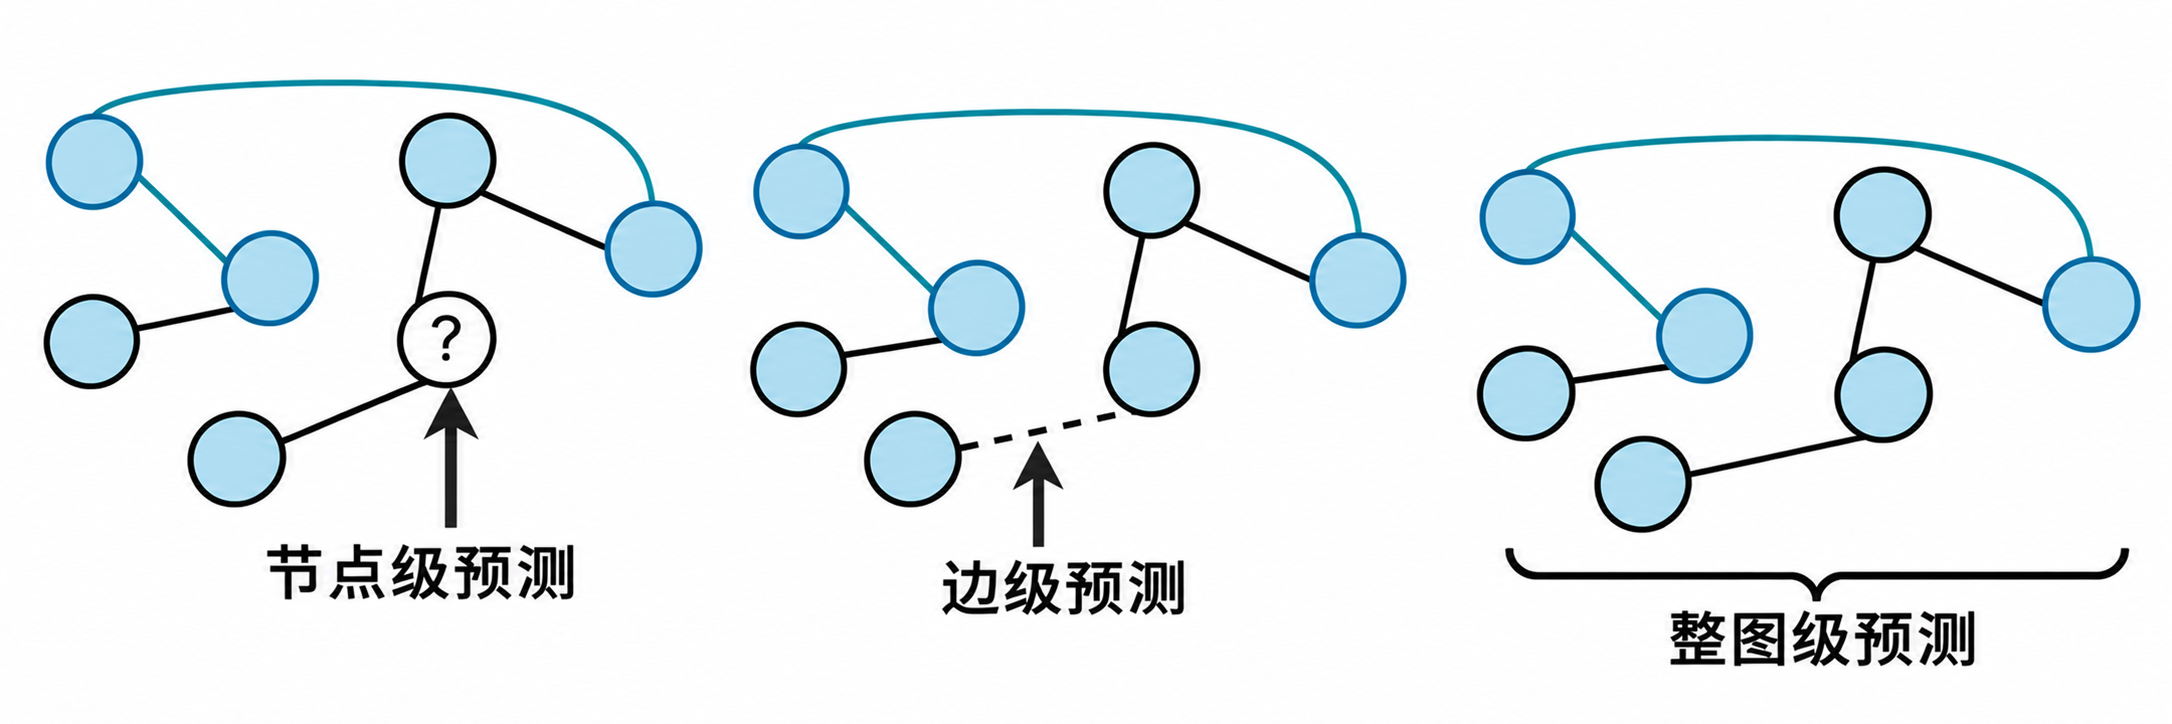
\includegraphics[width=\linewidth,height=0.34\textheight,keepaspectratio]{images/中文重绘/graph-tasks-cn.png}
\caption[节点级、边级与整图级任务]{节点级、边级与整图级任务\protect\footnotemark}
\label{fig:graph-task-levels}
\end{figure}
\footnotetext{来源：Khemani等，\href{https://doi.org/10.1186/s40537-023-00876-4}{\textit{A Review of Graph Neural Networks: Concepts, Architectures, Techniques, Challenges, Datasets, Applications, and Future Directions}}，2024，Figure 16。此处只采用该图对预测对象的区分。}

图神经网络（Graph Neural Network，GNN）是一类利用图结构学习表示的神经网络。图卷积网络（Graph Convolutional Network，GCN）是其中一种具体模型。GNN名称并不规定唯一的聚合公式，也不保证任意图上的预测都会改善。图中的边是否提供任务相关信息，要通过与只使用节点特征的模型比较来检验。

\section{消息传递的节点计算}
\subsection{从逐节点网络到邻域聚合}
若对每个节点独立使用同一个多层感知机，输出只依赖$\bm x_i$。这能共享参数，却没有使用连接关系。要让上游状态影响当前预测，可以让节点$j$先生成传给节点$i$的消息，再由节点$i$汇总所有消息。消息传递神经网络（Message Passing Neural Network，MPNN）给出一种通用表达\footnote{来源：Gilmer等，\href{https://arxiv.org/abs/1704.01212}{\textit{Neural Message Passing for Quantum Chemistry}}，2017。}：
\begin{align}
 \bm m_{i\leftarrow j}^{(\ell)}&=M_\ell(\bm h_i^{(\ell)},\bm h_j^{(\ell)},\bm e_{ij}),\label{eq:graph-message-function}\\
 \bm a_i^{(\ell)}&=\operatorname{AGG}_{j\in\mathcal N(i)}\bm m_{i\leftarrow j}^{(\ell)},\\
 \bm h_i^{(\ell+1)}&=U_\ell(\bm h_i^{(\ell)},\bm a_i^{(\ell)}).
 \label{eq:graph-message-passing}
\end{align}
$\bm e_{ij}$是边特征，例如流量或连接类型。$M_\ell$是消息函数，$\operatorname{AGG}$是聚合函数，$U_\ell$是更新函数。消息维度须一致才能相加，更新函数的输出为$d_{\ell+1}$维。这些函数可含可训练参数，同一层通常在节点间共享参数。

邻居没有天然的排列顺序。求和、均值和逐分量最大值均不依赖输入排列，但保留的信息不同。例如标量邻居特征的多重集$\{1,3\}$与$\{2,2\}$的均值都为$2$，均值聚合无法仅凭这个结果区分它们，二者的和也同为$4$。求和能反映数量，例如$\{2\}$与$\{2,2\}$的均值相同而和不同，但求和也会随节点度数改变尺度。选择聚合函数是在规定哪些邻域差异会保留下来。

一层读取一跳输入邻居，即沿一条允许的信息边向当前节点传递消息的节点。堆叠两层后，节点可以间接读取两跳输入邻居。若各层保留自身分支或自环，$L$层局部消息传递的计算依赖最多覆盖$L$跳范围，其中$L$为非负整数。有向图还要求路径方向与消息方向一致。这个范围只说明哪些输入可能进入计算，不保证每个输入对预测具有非零贡献，也不能据此确定故障的因果来源。没有全局操作时，有限层局部消息传递无法读取任意远处的信息。

\begin{figure}[htbp]
\centering
\begin{tikzpicture}[node distance=0.7cm and 0.8cm]
 \node[idi input] (neighbor) {邻居表示\\$\bm h_j^{(\ell)}$};
 \node[idi process,right=of neighbor] (message) {共享消息函数\\$M_\ell$};
 \node[idi state,right=of message] (aggregate) {无序邻域聚合\\$\bm a_i^{(\ell)}$};
 \node[idi output,right=of aggregate] (update) {节点更新\\$\bm h_i^{(\ell+1)}$};
 \node[idi input,below=of aggregate] (self) {自身表示\\$\bm h_i^{(\ell)}$};
 \draw[idi arrow] (neighbor)--(message);
 \draw[idi arrow] (message)--(aggregate);
 \draw[idi arrow] (aggregate)--(update);
 \draw[idi arrow] (self)--(update);
\end{tikzpicture}
\caption{消息传递将邻居信息的生成、汇总与节点更新分开。自身信息可通过更新函数进入，是否另加自环取决于具体模型。}
\label{fig:graph-message-passing}
\end{figure}

\subsection{节点编号与置换等变性}
节点重新编号不应改变设备关系。用置换矩阵$P\in\R^{n\times n}$重新排列节点时，特征变为$PH$，邻接矩阵变为$PAP^{\mathsf T}$。节点模型应满足置换等变性（permutation equivariance）：
\begin{equation}
 F(PAP^{\mathsf T},PH)=PF(A,H).
 \label{eq:graph-permutation-equivariance}
\end{equation}
即输出按相同顺序重新排列。共享参数与无序聚合可以实现这一性质。若随后对所有节点求和或取均值，整图表示在重新编号后保持不变，称为置换不变性。两者分别适合节点输出和整图输出，并不保证模型能区分所有不同的图结构。

\section{图卷积网络的矩阵计算}
\subsection{自环与对称归一化}
直接使用$AH$只汇总邻居，不包含自身。为使自身特征也进入聚合，取自环权重$\alpha>0$，定义
\begin{equation}
 \widetilde A=A+\alpha I_n,\qquad
 \widetilde d_i=\sum_j\widetilde A_{ij},\qquad
 \widetilde D=\diag(\widetilde d_1,\ldots,\widetilde d_n).
 \label{eq:graph-self-loop-degree}
\end{equation}
$I_n$是$n$阶单位矩阵，$\widetilde d_i$是加自环后的加权度数。标准GCN通常取$\alpha=1$。非负边权与正自环使$\widetilde d_i>0$，孤立节点也能计算逆平方根。原图若已有自环，该操作是在其上额外增加$\alpha$，须按实际对角元素计算。

直接求和会使高连接度节点累加更多信息。经典GCN使用对称归一化传播矩阵\footnote{来源：Kipf与Welling，\href{https://arxiv.org/abs/1609.02907}{\textit{Semi-Supervised Classification with Graph Convolutional Networks}}，2017。}：
\begin{equation}
 S=\widetilde D^{-1/2}\widetilde A\widetilde D^{-1/2},\qquad
 S_{ij}=\frac{\widetilde A_{ij}}{\sqrt{\widetilde d_i\widetilde d_j}}.
 \label{eq:graph-gcn-propagation}
\end{equation}
对角矩阵$\widetilde D^{-1/2}$的第$i$个对角元素为$1/\sqrt{\widetilde d_i}$。传播系数同时使用发送节点和接收节点的度数，且无向图的$S$保持对称。固定边权时，两端度数越大，该边的系数越小。

GCN的一层为
\begin{equation}
 H^{(\ell+1)}=\sigma\!\left(SH^{(\ell)}W^{(\ell)}\right),\qquad
 W^{(\ell)}\in\R^{d_\ell\times d_{\ell+1}}.
 \label{eq:graph-gcn-layer}
\end{equation}
$S$在节点之间传播信息，$W^{(\ell)}$在特征通道之间进行可训练变换，$\sigma$逐元素作用，例如整流线性单元（Rectified Linear Unit，ReLU）为$\max(0,z)$。维度依次为$(n\times n)(n\times d_\ell)(d_\ell\times d_{\ell+1})$，输出仍有$n$行。为突出传播，此处省略偏置，实际模型可在每行加入共享偏置。

对第$i$个节点，列向量形式为
\begin{equation}
 \bm h_i^{(\ell+1)}=\sigma\!\left(
 \sum_{j\in\mathcal N(i)\cup\{i\}}
 \frac{\widetilde A_{ij}}{\sqrt{\widetilde d_i\widetilde d_j}}
 W^{(\ell)\mathsf T}\bm h_j^{(\ell)}\right).
 \label{eq:graph-gcn-node}
\end{equation}
所有邻居使用同一个$W^{(\ell)}$。基本GCN的聚合系数由给定图结构确定，训练$W^{(\ell)}$不会自动学习每条边的权重。由结合律，$S(HW)=(SH)W$，在中间没有非线性或其他操作时，可以先聚合再变换，也可以先变换再聚合。

自环只是让自身参与混合，不保证原始特征完整保留。残差连接则在维度匹配时直接加上旧表示。二者计算不同。若去掉所有非线性，两层GCN变为$S^2XW^{(0)}W^{(1)}$，对输入仍是线性运算，因此非线性承担增加表达能力的作用。

\subsection{一个三节点路径的完整计算}
取无权路径$1-2-3$，每个节点只有一个特征，令$X=(1,2,3)^{\mathsf T}$、$\alpha=1$。于是
\begin{equation}
 A=\begin{bmatrix}0&1&0\\1&0&1\\0&1&0\end{bmatrix},\quad
 \widetilde A=\begin{bmatrix}1&1&0\\1&1&1\\0&1&1\end{bmatrix},\quad
 \widetilde D=\diag(2,3,2).
\end{equation}
三个节点加自环后的度数分别为$2,3,2$。代入式\eqref{eq:graph-gcn-propagation}得到
\begin{equation}
 S=\begin{bmatrix}
 1/2&1/\sqrt6&0\\
 1/\sqrt6&1/3&1/\sqrt6\\
 0&1/\sqrt6&1/2
 \end{bmatrix}.
\end{equation}
暂取$W=1$与恒等激活，只观察图传播：
\begin{equation}
 SX=\begin{bmatrix}1/2+2/\sqrt6\\4/\sqrt6+2/3\\2/\sqrt6+3/2\end{bmatrix}
 \approx\begin{bmatrix}1.3165\\2.2997\\2.3165\end{bmatrix}.
 \label{eq:graph-path-example}
\end{equation}
节点$1$只使用自身和节点$2$。节点$3$要经第二层才能影响节点$1$。图\ref{fig:graph-gcn-local-calculation}展开节点$1$的两项输入。自环与邻边的系数不同，来自加自环后的度数。虚线标出的第二层路径解释节点$3$的信息何时才能到达节点$1$。
\begin{figure}[htbp]
\centering
\begin{tikzpicture}[node distance=0.65cm and 1cm]
 \node[idi input] (self) at (0,1) {自身：$x_1=1$};
 \node[idi input] (neighbor) at (0,-0.5) {邻居：$x_2=2$};
 \node[idi state] (sum) at (4,0.25) {相加\\$\frac12+\frac2{\sqrt6}$};
 \node[idi output] (out) at (7,0.25) {$h_1'=1.3165$};
 \draw[idi arrow] (self)--node[above,font=\small] {$\times1/2$} (sum);
 \draw[idi arrow] (neighbor)--node[below,font=\small] {$\times1/\sqrt6$} (sum);
 \draw[idi arrow] (sum)--(out);
 \node[font=\small] (third) at (0,-1.8) {节点3};
 \node[font=\small] (second) at (3,-1.8) {节点2};
 \node[font=\small] (first) at (6,-1.8) {节点1};
 \draw[idi feedback] (third)--node[above,font=\scriptsize] {第一层} (second);
 \draw[idi feedback] (second)--node[above,font=\scriptsize] {第二层} (first);
\end{tikzpicture}
\caption{GCN路径算例中节点1的局部计算，取$W=1$与恒等激活。实线箭头表示本层计算，底部虚线箭头表示跨两层的信息路径，不表示该信息一定改善预测。}
\label{fig:graph-gcn-local-calculation}
\end{figure}

第一行系数和约为$0.9082$，第二行约为$1.1498$，说明对称归一化一般不等于邻居平均。

若目标是严格的加权平均，可以使用按行归一化的$R=\widetilde D^{-1}\widetilde A$。其每行系数和为一，$RX$在本例中为$(1.5,2,2.5)^{\mathsf T}$。$R$与$S$是不同的传播设计，不能将平均的解释直接套到式\eqref{eq:graph-gcn-layer}。

\subsection{带权边、方向与自环尺度}
若两条路径边的权重改为$2$和$1$，则
\begin{equation}
 A=\begin{bmatrix}0&2&0\\2&0&1\\0&1&0\end{bmatrix},\qquad
 \widetilde D=\diag(3,4,2).
\end{equation}
度数由边权求和，不能继续使用邻居数量。仍取$X=(1,2,3)^{\mathsf T}$，对称归一化后节点$2$的结果为
\begin{equation}
 (SX)_2=\frac2{\sqrt{12}}\times1+\frac14\times2+\frac1{\sqrt8}\times3
 \approx2.1380.
\end{equation}
按行归一化的结果则为$(2\times1+1\times2+1\times3)/4=1.75$。较大的原始边权不必对应较大的最终贡献，贡献还包含度数、输入特征和特征变换。

边权应表示传播强度。若原始数值是距离，较大距离通常不应带来更强传播，可用$A_{ij}=\exp[-\operatorname{dist}(i,j)^2/(2s^2)]$转换，$s>0$为与距离同单位的尺度，再按需要限制邻域。距离定义、尺度和截断规则均属于建图假设，应在训练与验证协议内确定。

将包括自环在内的全部边权乘以$c>0$时，归一化中的$c$相消，$S$不变。只放大$A$而固定$\alpha$会改变自身与邻居的相对贡献。自环权重应结合原始边权尺度选择。

有向关系需要保留信息流方向。按本章约定，$A_{ij}$表示$j$向$i$传递信息。若原始记录把$A_{ij}$定义为从$i$到$j$的连接，应先转置或重定义传播。入边与出边还可以使用不同通道。此时无向图的对称谱推导不再直接适用。带符号边权的求和可能得到零或负度数，不能直接套用实数逆平方根。正负关系需要分开传播或采用专门的符号图模型。

\section{图卷积的谱滤波解释}
图像卷积按固定相对位置共享核权重，图的邻居通常没有统一的左右顺序。经典GCN不为每个邻居位置学习不同的核，因此即使把图像看作网格图，GCN也不自动等价于任意二维卷积。图卷积名称的另一层依据来自频率滤波。

\subsection{图拉普拉斯与图频率}
普通有限信号的循环卷积满足傅里叶变换后的逐频率相乘关系。图上没有一般的平移操作，可以用图拉普拉斯矩阵的特征向量建立信号基。暂用加自环前的无向非负图，并假设每个节点度数$d_i=\sum_jA_{ij}>0$，定义
\begin{equation}
 \begin{aligned}
 D&=\diag(d_1,\ldots,d_n),\\
 L_G&=I_n-D^{-1/2}AD^{-1/2}=U\Lambda U^{\mathsf T}.
 \end{aligned}
 \label{eq:graph-laplacian}
\end{equation}
$L_G$是对称归一化图拉普拉斯矩阵。$U$的列为正交单位特征向量，满足$U^{\mathsf T}U=I_n$。对角矩阵$\Lambda$记录特征值$\lambda_1,\ldots,\lambda_n$。孤立节点可单独处理，不能在本式中直接取零度数的逆。

对标量节点信号$\bm x\in\R^n$，展开二次型得到
\begin{align}
 \bm x^{\mathsf T}L_G\bm x
 &=\sum_i x_i^2-\sum_{i,j}A_{ij}\frac{x_ix_j}{\sqrt{d_id_j}}\\
 &=\frac12\sum_{i,j}A_{ij}\left(\frac{x_i}{\sqrt{d_i}}-\frac{x_j}{\sqrt{d_j}}\right)^2.
 \label{eq:graph-smoothness}
\end{align}
第二步使用$A$对称及$\sum_jA_{ij}=d_i$。该量衡量相连节点的度数调整后信号差异。单位特征向量$\bm u_k$满足$\bm u_k^{\mathsf T}L_G\bm u_k=\lambda_k$，故小特征值对应沿边缓慢变化的模式，大特征值对应变化较强的模式。这里的平滑不要求原始$x_i$都相等。

图傅里叶变换为$\widehat{\bm x}=U^{\mathsf T}\bm x$，逆变换为$\bm x=U\widehat{\bm x}$。谱图卷积定义为
\begin{equation}
 g_\theta *_G\bm x=Ug_\theta(\Lambda)U^{\mathsf T}\bm x,
 \qquad g_\theta(\Lambda)=\diag(g_\theta(\lambda_1),\ldots,g_\theta(\lambda_n)).
 \label{eq:graph-spectral-filter}
\end{equation}
$g_\theta(\lambda_k)$是滤波器对第$k$个模式的响应。计算先变换到图频率，再分别缩放，最后返回节点域。任意谱响应可能涉及全图，局部性还需要约束滤波器形式。

\subsection{多项式、一阶近似与重归一化}
直接特征分解成本较高。可以用拉普拉斯多项式近似滤波器，切比雪夫图滤波是一个代表\footnote{来源：Defferrard、Bresson与Vandergheynst，\href{https://arxiv.org/abs/1606.09375}{\textit{Convolutional Neural Networks on Graphs with Fast Localized Spectral Filtering}}，2016。}：
\begin{equation}
 g_\theta *_G\bm x\approx\sum_{k=0}^K\theta_kT_k(\overline L_G)\bm x,\qquad
 \overline L_G=\frac2{\lambda_{\max}}L_G-I_n.
\end{equation}
$K$是多项式阶数，$\lambda_{\max}>0$为最大特征值，缩放使谱落在$[-1,1]$。切比雪夫多项式满足$T_0(z)=1$、$T_1(z)=z$、$T_{k+1}(z)=2zT_k(z)-T_{k-1}(z)$。矩阵版本可递推计算，不必显式求$U$。$L_G$只有对角与相邻节点处可能非零，因此$K$阶多项式最多传播到$K$跳邻域。

取$K=1$，并采用归一化拉普拉斯的上界$2$近似$\lambda_{\max}$，得到
\begin{align}
 g_\theta *_G\bm x
 &\approx\theta_0\bm x+\theta_1(L_G-I_n)\bm x\\
 &=\theta_0\bm x-\theta_1D^{-1/2}AD^{-1/2}\bm x.
\end{align}
该图的最大特征值未必等于$2$，所以第一步包含近似。进一步约束$\theta_0=\theta$、$\theta_1=-\theta$，得到$\theta(I_n+D^{-1/2}AD^{-1/2})\bm x$。这些选择减少参数，也限制了可表达的滤波器。

经典GCN随后采用$\alpha=1$的重归一化替换：
\begin{equation}
 I_n+D^{-1/2}AD^{-1/2}\quad\longrightarrow\quad
 \widetilde D^{-1/2}(A+I_n)\widetilde D^{-1/2}=S.
\end{equation}
这是设计替换，通常不是等式。前者的特征值可达到$2$，反复传播可能放大某些方向。后者在无向非负图与正自环条件下的特征值绝对值不超过$1$，从而控制图传播本身的尺度。可训练矩阵$W$仍可能放大特征，不能据此保证整个网络稳定。

将标量信号推广到多通道、加入可训练特征变换和非线性，就得到式\eqref{eq:graph-gcn-layer}。在最终加自环图上定义$\widetilde L_G=I_n-S$，则$S=I_n-\widetilde L_G$也是该图拉普拉斯的一阶滤波。任意消息传递模型未必能写成这种谱滤波形式。

\section{固定邻域聚合留下的两个问题}
\subsection{大图与新节点：邻域采样}
整图GCN在一层中读取所有相关边。大图训练时，多层邻域展开可能带来较高存储成本。图采样与聚合方法（Graph Sample and Aggregate，GraphSAGE）通过学习共享邻域函数并采样邻居处理这一问题。一种均值版本为
\begin{equation}
 \bm h_i^{(\ell+1)}=\sigma\!\left(B_\ell
 \begin{bmatrix}\bm h_i^{(\ell)}\\
 |\mathcal S_\ell(i)|^{-1}\sum_{j\in\mathcal S_\ell(i)}\bm h_j^{(\ell)}
 \end{bmatrix}+\bm b_\ell\right).
\end{equation}
$\mathcal S_\ell(i)\subseteq\mathcal N(i)$是本次采样的邻居集合，$B_\ell\in\R^{d_{\ell+1}\times2d_\ell}$将自身与邻居均值的拼接映射到输出。上式只展示$\mathcal S_\ell(i)\ne\varnothing$的情形。若邻域为空，不能把零代入分母。应直接把邻居聚合定义为$\bm0\in\R^{d_\ell}$，再保留自身分支完成更新。拼接保留了自身与邻居的来源区别。

若从非空邻域中等概率抽取固定数量的邻居，样本特征均值是完整邻居均值的无偏估计。这里的无偏性只针对聚合前的均值。经过非线性更新与多层复合后，节点表示通常不是完整邻域计算结果的无偏估计。采样降低单次计算量，同时引入随机性。推理应说明使用完整邻域还是采样，以及是否重复采样。

图\ref{fig:graph-graphsage-original}先从目标节点向外采样多跳邻域，再按层从采样到的外层节点向目标节点汇总。图中$k=1$、$k=2$表示距目标节点一跳、两跳的采样范围，对应两层聚合。第三栏同时画出图上下文与节点标签，是原论文无监督目标和监督目标的示例。实际训练按可用监督选择目标，并非每次使用GraphSAGE都要同时预测二者。图中出现的节点是本次更新的计算依赖，不表示它们都具有预测标签，也不证明沿边存在因果影响。

\Needspace{.40\textheight}
\begin{figure}[H]
\centering
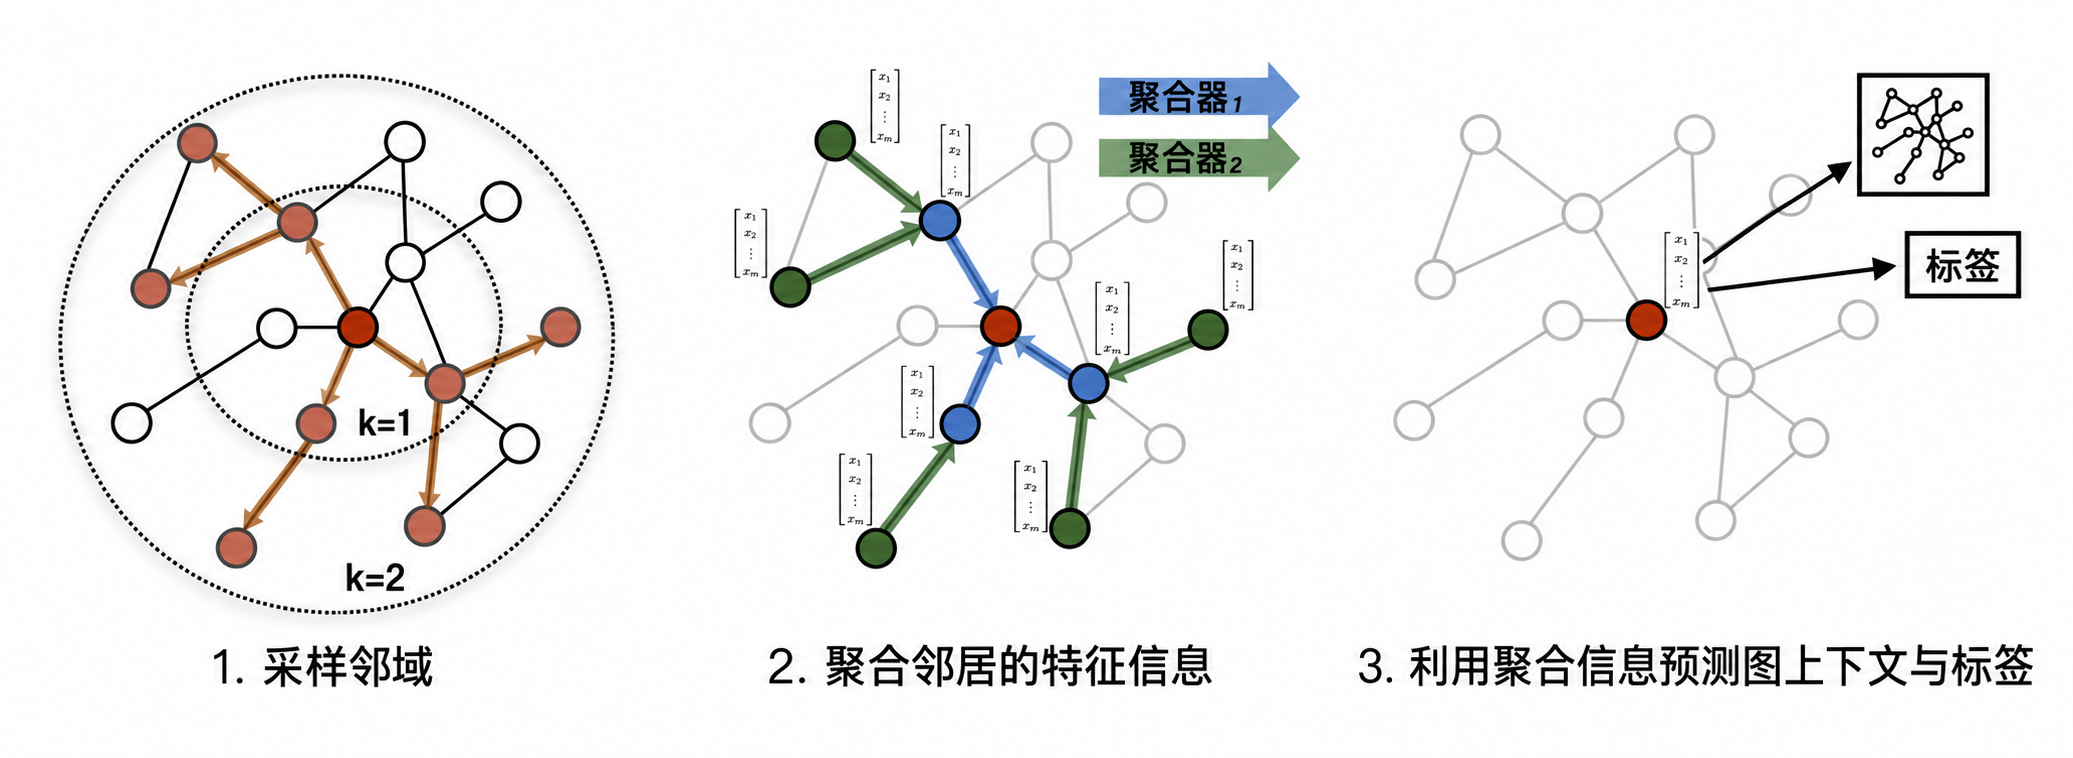
\includegraphics[width=\linewidth,height=0.36\textheight,keepaspectratio]{images/中文重绘/graphsage-cn.png}
\caption[GraphSAGE的邻域采样与逐层聚合]{GraphSAGE的邻域采样与逐层聚合\protect\footnotemark}
\label{fig:graph-graphsage-original}
\end{figure}
\footnotetext{来源：Hamilton、Ying与Leskovec，\href{https://arxiv.org/abs/1706.02216v4}{\textit{Inductive Representation Learning on Large Graphs}}，2017，Figure 1（PDF第2页）。}

共享函数可应用于新节点，前提是新节点具有兼容特征与可用关系。这称为归纳式使用。它不保证新工厂分布下的泛化。GCN同样可以在新图上使用共享参数，归纳或传导设定取决于数据与验证协议，不能仅按模型名字区分。

\subsection{特征驱动的图注意力}
GCN的系数由边权和度数决定。当同一设备的不同邻居在不同工况下作用不同，可以让特征参与聚合系数的计算。图注意力网络（Graph Attention Network，GAT）的一种单头形式为
\begin{align}
 \bm z_i&=B\bm h_i,\label{eq:graph-attention-proj}\\
 e_{ij}&=\operatorname{LeakyReLU}\!\left(\bm a^{\mathsf T}[\bm z_i\Vert\bm z_j]\right),\\
 \beta_{ij}&=\frac{\exp(e_{ij})}{\sum_{k\in\mathcal N(i)\cup\{i\}}\exp(e_{ik})},\label{eq:graph-attention-coef}\\
 \bm h_i'&=\sigma\!\left(\sum_{j\in\mathcal N(i)\cup\{i\}}\beta_{ij}\bm z_j\right).
 \label{eq:graph-attention}
\end{align}
$B\in\R^{d'\times d_\ell}$与$\bm a\in\R^{2d'}$为可训练参数，$\Vert$表示拼接。带泄漏的整流函数使用固定$0<\eta<1$，定义为
\[
 \operatorname{LeakyReLU}(u)=\max(u,\eta u).
\]
归一化在接收节点$i$的邻域内完成，故$\sum_j\beta_{ij}=1$，但一般$\beta_{ij}\ne\beta_{ji}$，也不同于GCN的对称归一化。

例如候选集合只含节点$i$自身和一个邻居，二者得分依次为$\log2$和$0$，对应系数为$2/3$和$1/3$。自身与邻居共同进入同一个softmax分母。它们由输入与参数计算，随训练和样本改变。多头注意力用多组独立参数计算，再拼接或平均。注意力不会自动发现候选边以外的关系，权重大小也不能直接解释为故障原因。

图\ref{fig:graph-gat-original}左侧展开接收节点与邻居之间的注意力得分，softmax只在该接收节点的候选邻域内比较。原图中的$W$和$\alpha_{ij}$分别对应式\eqref{eq:graph-attention-proj}中的$B$和式\eqref{eq:graph-attention-coef}中的$\beta_{ij}$。右侧用$K=3$演示三组独立注意力头。隐藏层常拼接各头结果，输出层可以取平均。图中的颜色和线型用于区分注意力头，不表示权重大小，三个头也只是结构示例。

\Needspace{.46\textheight}
\begin{figure}[H]
\centering
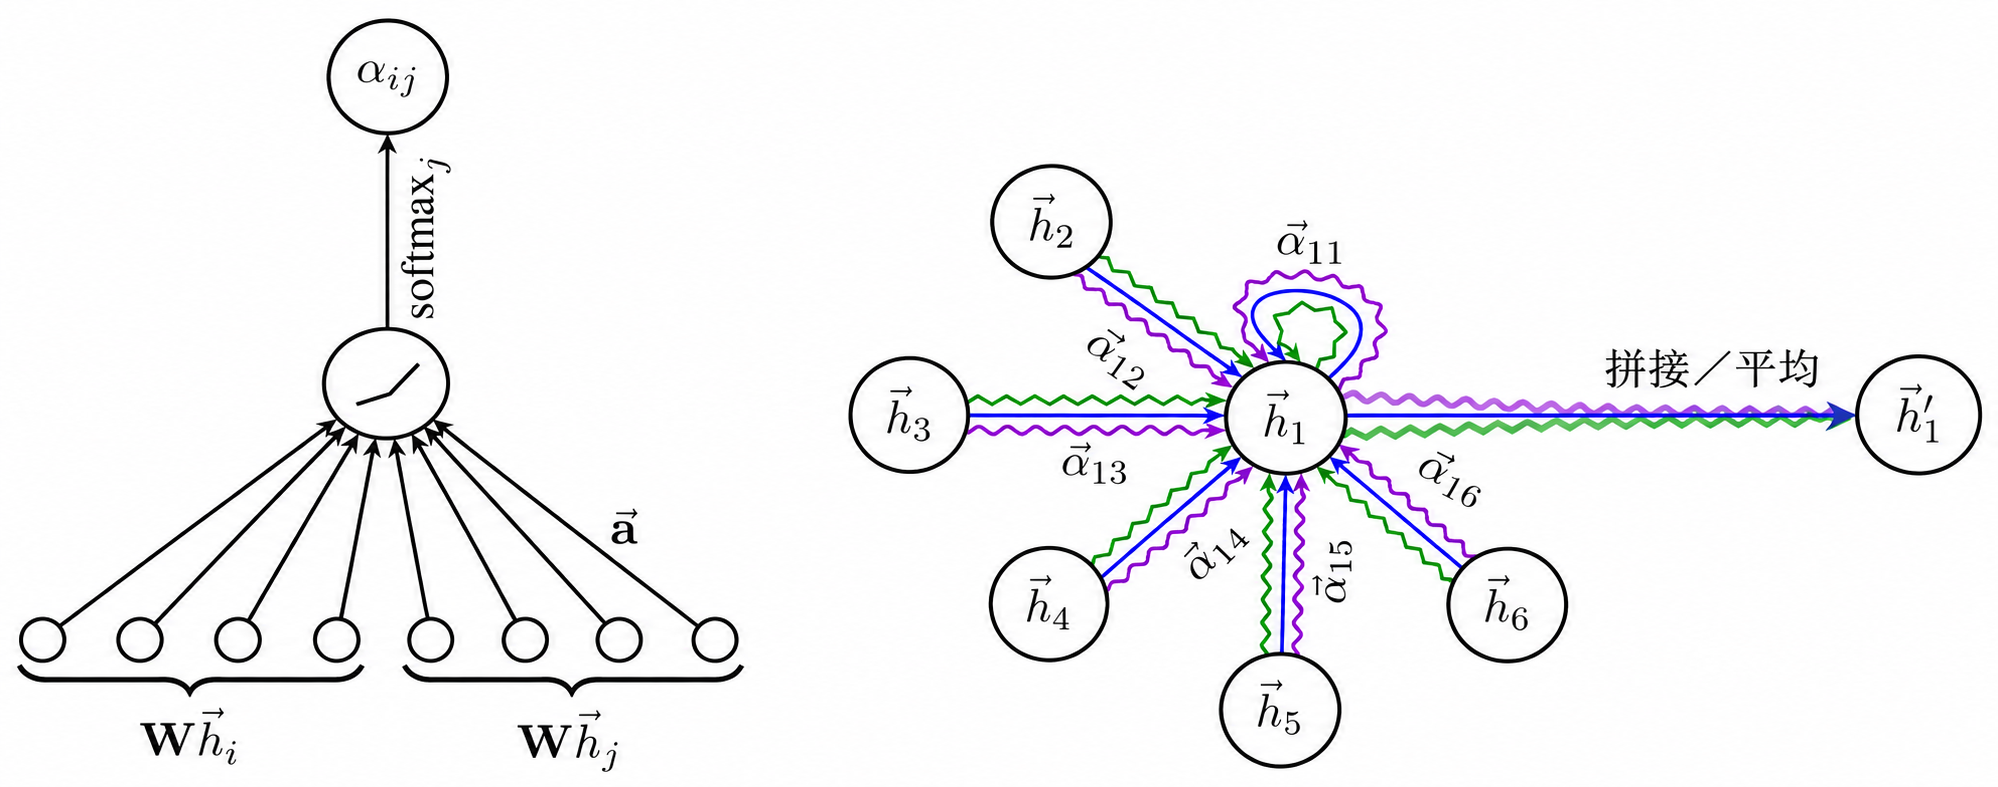
\includegraphics[width=\linewidth,height=0.40\textheight,keepaspectratio]{images/中文重绘/gat-cn.png}
\caption[GAT的邻域注意力与多头聚合]{GAT的邻域注意力与多头聚合\protect\footnotemark}
\label{fig:graph-gat-original}
\end{figure}
\footnotetext{来源：Veli\v{c}kovi\'{c}等，\href{https://arxiv.org/abs/1710.10903v3}{\textit{Graph Attention Networks}}，2018，Figure 1（PDF第4页）。}

\section{超图与共同参与关系}
\subsection{成对连接与组身份}
普通图的一条边连接两个节点。若三台设备共同执行一次工序，只记录三条成对边，会丢掉“它们属于同一次共同参与关系”的身份。超图（hypergraph）允许一条超边（hyperedge）连接任意非空节点子集，可用来记录共同工序、共享供电组或一次已知的联合操作。

例如$\{1,2,3\}$这一条超边，与$\{1,2\},\{2,3\},\{1,3\}$三条超边表示不同的组关系。将二者都简单变成同一个三角形，无法恢复原始分组。使用超图的理由应来自组关系的含义，不能仅因参与节点多就断言它比普通图更适合。

设有$m$条超边$\mathcal E_H=\{e_1,\ldots,e_m\}$，用关联矩阵$C\in\{0,1\}^{n\times m}$表示：
\begin{equation}
 C_{ir}=\begin{cases}1,&i\in e_r,\\0,&i\notin e_r.\end{cases}
 \label{eq:graph-hyper-incidence}
\end{equation}
第$i$行记录节点参加哪些组，第$r$列记录超边包含哪些节点。此处用$C$避免与隐藏特征矩阵$H^{(\ell)}$混淆。为每条超边指定正权重$\omega_r>0$，定义
\begin{equation}
 \begin{aligned}
 \Omega&=\diag(\omega_1,\ldots,\omega_m),&
 \delta_r&=\sum_iC_{ir},&
 d_i^H&=\sum_r\omega_rC_{ir},\\
 D_e&=\diag(\delta_1,\ldots,\delta_m),&
 D_v&=\diag(d_1^H,\ldots,d_n^H).
 \end{aligned}
 \label{eq:graph-hyper-degrees}
\end{equation}
$\delta_r$是超边大小，$d_i^H$是节点参加的超边权重之和。以下假设没有空超边且每个节点至少参加一条超边，从而逆矩阵有定义。孤立节点可增加只含自身的单节点超边，或通过独立自身通道处理，不能直接计算零度数的逆。

图\ref{fig:graph-hyper-incidence-picture}把关联矩阵的每个非零元素画成一条成员关系。这里将超边画成单独的方框，便于区分组身份。方框不是新增的物理设备，线段也不是设备之间的管路。
\begin{figure}[htbp]
\centering
\begin{tikzpicture}
 \node[idi input] (n1) at (0,1.4) {节点1};
 \node[idi input] (n2) at (0,0) {节点2};
 \node[idi input] (n3) at (0,-1.4) {节点3};
 \node[idi process] (e1) at (3,0.8) {$e_1=\{1,2,3\}$};
 \node[idi process] (e2) at (3,-0.8) {$e_2=\{2,3\}$};
 \draw[thick] (n1)--(e1);
 \draw[thick] (n2)--(e1); \draw[thick] (n3)--(e1);
 \draw[thick,dashed] (n2)--(e2); \draw[thick,dashed] (n3)--(e2);
 \node[align=center] at (7,0) {$C=\begin{bmatrix}1&0\\1&1\\1&1\end{bmatrix}$\\[4pt]\small 行：节点1、2、3\\\small 列：超边$e_1,e_2$};
\end{tikzpicture}
\caption{超图的节点--超边关联表示。实线为第一组的成员关系，虚线为第二组的成员关系，均无方向。节点2与3各参加两个组，节点1只参加第一组。}
\label{fig:graph-hyper-incidence-picture}
\end{figure}

\subsection{从节点到超边，再从超边到节点}
先让每条超边取参与节点的均值，再让节点按超边权重汇总组表示：
\begin{equation}
 Q=D_e^{-1}C^{\mathsf T}H\in\R^{m\times d},\qquad
 H'=D_v^{-1}C\Omega Q=R_HH,
 \quad R_H=D_v^{-1}C\Omega D_e^{-1}C^{\mathsf T}.
 \label{eq:graph-hyper-random-walk}
\end{equation}
$Q$每行是一条超边的特征。第一步除以组大小，避免大组仅因成员多而产生更大和。第二步除以节点超边度数。矩阵的节点系数为
\begin{equation}
 (R_H)_{ij}=\frac1{d_i^H}\sum_{r:i,j\in e_r}\frac{\omega_r}{\delta_r}.
\end{equation}
它表示节点$i$先以$\omega_r/d_i^H$选择一条自己参加的超边，再以$1/\delta_r$选择该超边中的节点$j$。因此各行系数和为一。该解释依赖正权重与上述覆盖条件。

超图神经网络（Hypergraph Neural Network，HGNN）的经典对称归一化卷积采用\footnote{来源：Zhou、Huang与Sch\"olkopf，\href{https://proceedings.neurips.cc/paper_files/paper/2006/hash/dff8e9c2ac33381546d96deea9922999-Abstract.html}{\textit{Learning with Hypergraphs: Clustering, Classification, and Embedding}}，2006。Feng等，\href{https://arxiv.org/abs/1809.09401}{\textit{Hypergraph Neural Networks}}，2019。}
\begin{equation}
 S_H=D_v^{-1/2}C\Omega D_e^{-1}C^{\mathsf T}D_v^{-1/2},\qquad
 H^{(\ell+1)}=\sigma\!\left(S_HH^{(\ell)}W^{(\ell)}\right).
 \label{eq:graph-hyper-convolution}
\end{equation}
$S_H\in\R^{n\times n}$，$W^{(\ell)}\in\R^{d_\ell\times d_{\ell+1}}$。从右向左读，先对节点特征作度数缩放，再汇总到超边、除以组大小、乘超边权重、返回节点，最后再次作节点度数缩放。特征变换与逐元素非线性随后产生新表示。

节点形式进一步说明每条超边的贡献：
\begin{equation}
 \bm h_i^{(\ell+1)}=\sigma\!\left(
 \sum_{r:i\in e_r}\sum_{j\in e_r}
 \frac{\omega_r}{\delta_r\sqrt{d_i^Hd_j^H}}
 W^{(\ell)\mathsf T}\bm h_j^{(\ell)}\right).
 \label{eq:graph-hyper-node}
\end{equation}
一条超边使其中所有节点在本层交换信息。两个节点若共同参加多条超边，系数会累加。自身也属于这些组，所以$S_H$已有正对角项，通常无需为模仿GCN再机械添加单位矩阵。额外添加单节点超边会改变度数和传播，需要明确其目的。

\subsection{三个节点、两条超边的手算}
令$e_1=\{1,2,3\}$、$e_2=\{2,3\}$，超边权重均为$1$。取$X=(1,2,3)^{\mathsf T}$，则
\begin{equation}
 C=\begin{bmatrix}1&0\\1&1\\1&1\end{bmatrix},\qquad
 D_e=\diag(3,2),\qquad D_v=\diag(1,2,2).
\end{equation}
第一条组均值为$(1+2+3)/3=2$，第二条为$(2+3)/2=2.5$。按行归一化传播中，节点$1$只参加第一组，输出$2$。节点$2,3$参加两组，输出$(2+2.5)/2=2.25$。

图\ref{fig:graph-hyper-two-stage}展开两次平均的具体计算。左右两列表示同一批节点在更新前后的值，中间两行是组表示。节点$2$与$3$读取相同的组，所以这一传播会得到相同输出。
\begin{figure}[htbp]
\centering
\begin{tikzpicture}
 \node[idi input] (a) at (0,1.6) {$x_1=1$};
 \node[idi input] (b) at (0,0) {$x_2=2$};
 \node[idi input] (c) at (0,-1.6) {$x_3=3$};
 \node[idi process] (p) at (4,0.9) {$q_1=(1+2+3)/3=2$};
 \node[idi process] (q) at (4,-0.9) {$q_2=(2+3)/2=2.5$};
 \node[idi output] (u) at (8,1.6) {$x_1'=q_1=2$};
 \node[idi output] (v) at (8,0) {$x_2'=(q_1+q_2)/2=2.25$};
 \node[idi output] (w) at (8,-1.6) {$x_3'=(q_1+q_2)/2=2.25$};
 \draw[idi arrow] (a)--(p); \draw[idi arrow] (b)--(p); \draw[idi arrow] (c)--(p);
 \draw[idi arrow,dashed] (b)--(q); \draw[idi arrow,dashed] (c)--(q);
 \draw[idi arrow] (p)--(u); \draw[idi arrow] (p)--(v); \draw[idi arrow] (p)--(w);
 \draw[idi arrow,dashed] (q)--(v); \draw[idi arrow,dashed] (q)--(w);
 \node[font=\small] at (2,2.4) {节点到组：成员平均};
 \node[font=\small] at (6,2.4) {组到节点：参与组平均};
\end{tikzpicture}
\caption{权重均为1的超图行归一化传播$R_HX$。实线箭头经第一组，虚线箭头经第二组。本图展示两次普通平均，不是对称归一化$S_HX$的计算图。}
\label{fig:graph-hyper-two-stage}
\end{figure}

对称归一化则给出
\begin{equation}
 S_H=\begin{bmatrix}
 1/3&1/(3\sqrt2)&1/(3\sqrt2)\\
 1/(3\sqrt2)&5/12&5/12\\
 1/(3\sqrt2)&5/12&5/12
 \end{bmatrix}.
\end{equation}
暂取$W=1$和恒等激活，得到
\begin{equation}
 S_HX=\begin{bmatrix}1/3+5/(3\sqrt2)\\1/(3\sqrt2)+25/12\\1/(3\sqrt2)+25/12\end{bmatrix}
 \approx\begin{bmatrix}1.5118\\2.3190\\2.3190\end{bmatrix}.
 \label{eq:graph-hyper-example}
\end{equation}
对称归一化与两次普通平均不相同。节点$2,3$参与的组完全相同，在这个线性传播例子中得到相同结果，原先的特征差异被汇总消去。加入自身残差通道可以保留这类差异，但不能保证任意组结构下都获得更好的预测。

\subsection{超图拉普拉斯与成对传播的联系}
定义超图拉普拉斯$L_H=I_n-S_H$，对$\bm x\in\R^n$可展开为
\begin{equation}
 \bm x^{\mathsf T}L_H\bm x=
 \frac12\sum_{r=1}^m\frac{\omega_r}{\delta_r}
 \sum_{i,j\in e_r}
 \left(\frac{x_i}{\sqrt{d_i^H}}-\frac{x_j}{\sqrt{d_j^H}}\right)^2.
 \label{eq:graph-hyper-smoothness}
\end{equation}
对每条超边展开平方，利用$\delta_r=|e_r|$和$\sum_r\omega_rC_{ir}=d_i^H$，平方项合计为$\sum_i x_i^2$，交叉项为$\bm x^{\mathsf T}S_H\bm x$，得到本式。它惩罚同一组内的度数调整后差异。$S_H$也可写成$BB^{\mathsf T}$，其中$B=D_v^{-1/2}C\Omega^{1/2}D_e^{-1/2}$，故为半正定矩阵。由$S_H=D_v^{1/2}R_HD_v^{-1/2}$，二者具有相同的特征值。$R_H$为非负行随机矩阵，特征值绝对值不超过$1$。再结合$S_H$半正定，得到其特征值位于$[0,1]$，可在此基础上定义谱滤波。

关联矩阵保留了组身份，但上述线性卷积对特征的作用可等价地写成一个成对图算子。令
\begin{equation}
 A_* =C\Omega D_e^{-1}C^{\mathsf T},\qquad
 (A_*)_{ij}=\sum_{r:i,j\in e_r}\frac{\omega_r}{\delta_r}.
 \label{eq:graph-hyper-clique}
\end{equation}
该矩阵包含自连接，行和为$d_i^H$，因此$S_H=D_v^{-1/2}A_*D_v^{-1/2}$。这说明经典线性HGNN传播可以视为带特定权重与自连接的成对图传播。不能仅凭采用超图公式，就宣称网络能表达任意不可分解的高阶相互作用。

若任务需要在组内先进行非线性计算，可保留显式超边表示：
\begin{equation}
 \bm q_r=\phi_e\!\left(\operatorname{AGG}_{j\in e_r}\phi_v(\bm h_j),\bm u_r\right),\qquad
 \bm h_i'=\psi\!\left(\bm h_i,\operatorname{AGG}_{r:i\in e_r}\bm q_r\right).
\end{equation}
$\bm u_r$为超边属性，例如工序类型，$\phi_v,\phi_e,\psi$为共享可训练函数。节点到超边之间的非线性与组属性能保留更多组级计算，通常无法直接合并成一个固定$A_*$。具体表达能力仍依赖聚合函数与数据，不能由结构名称单独保证。

\section{图模型训练与信息边界}
\subsection{从节点表示到故障概率与训练损失}
回到设备预测任务。设最后一层宽度为$d_L$，输出矩阵$W_o\in\R^{d_L\times2}$，则
\begin{equation}
 Z=H^{(L)}W_o+\bm1_n\bm b_o^{\mathsf T}\in\R^{n\times2},\qquad
 p_{ic}=\frac{\exp(Z_{ic})}{\exp(Z_{i0})+\exp(Z_{i1})},\quad c\in\{0,1\}.
\end{equation}
$\bm b_o\in\R^2$是偏置，$\bm1_n$是全一列向量。每行的两个实数得分在类别轴上归一化，$p_{i1}$表示模型输出的故障概率，不能在全部节点间做一次softmax。设训练标签集合为非空的$\mathcal V_{\rm tr}$，$y_i\in\{0,1\}$，经验目标为
\begin{equation}
 \mathcal L_{\rm tr}=-\frac1{|\mathcal V_{\rm tr}|}\sum_{i\in\mathcal V_{\rm tr}}\log p_{i,y_i}
 +\lambda\sum_\ell\|W^{(\ell)}\|_F^2,\qquad\lambda\geq0.
\end{equation}
$\|\cdot\|_F$为矩阵元素平方和的平方根。第一项是训练节点的交叉熵，第二项限制部分参数的大小，是否包含输出矩阵应在实现中规定。验证与测试标签不参与参数梯度更新，也不作为建图或标准化的输入。验证标签可用于选择超参数和决策阈值，测试标签只用于最终评价。图使输出相互依赖，这一经验目标不意味着节点标签在真实系统中独立。

训练时梯度穿过传播、特征变换和输出头更新参数。给定固定图时，$A$或$C$不会因训练上述矩阵而自动改变。推理时固定参数，根据当前可用特征与图前向计算。多次预测形成训练样本时，还须按时间组织图快照与标签窗口。

整图回归可先用$\bm r=n^{-1}\sum_i\bm h_i^{(L)}$汇聚，再用回归头输出一个量。均值读出不直接保留节点的多重性，求和读出对节点数量和表示总量更敏感。节点表示本身仍可能已经编码度数与拓扑，不能据此断言均值完全忽略图规模\footnote{相关讨论参见Xu等，\href{https://arxiv.org/abs/1810.00826}{\textit{How Powerful Are Graph Neural Networks?}}，2019。}。应按目标含义选择读出。边预测可用两端表示的拼接作为输入，若任务要求无向边概率，应使用对称打分或显式对称化。

做边预测时，用于验证或测试的目标边以及预测时刻尚未发生的边，不能同时作为当次输入图中的已知连接，应在划分与构图时隔离。目标边的隔离规则取决于任务：若预测未来新边，应按时间划分并确保输入图只含预测时刻前已观测的边。若评估同一静态图中隐藏边的重构，可在明确掩码与负采样规则后使用其余训练边。两种设定都不能把目标边本身传入模型。

\subsection{传导设定与归纳设定}
传导式学习（transductive learning）可以在训练时使用同一张固定图中无标签测试节点的特征与连接，只对训练节点计损失。前提是这些无标签信息在部署设定中确实可用，且协议明确允许。测试标签始终不能进入传播或建图。

归纳式学习（inductive learning）在测试时遇到训练阶段未见的节点或整张图，例如新工厂的设备系统。应完整留出这些设备或系统，而不是仅隐藏其标签。若目标是预测未来，训练阶段还不能读取未来节点观测、未来连接或未来共同工序。使用预测时已知的计划关系时，应与事后执行记录区分，并检验计划变更的影响。

图可来自已知物理连接，也可来自特征相似度。按本章的预处理约定，标准化统计量只在训练数据上拟合，固定后再应用于验证与测试数据。距离尺度、最近邻数量和相似度阈值可借验证集选择。用全时间段相关性建图，再宣称模型能提前预测，会把未来信息引入输入。连接可以反映统计相关性，但相关边和注意力系数都不是因果关系的证明。

\section{传播失效与验证}
\subsection{同配关系与过平滑}
相连节点倾向具有相似标签或属性，称为同配性（homophily）。GCN的平滑倾向常在这种结构下有用。工业图中，上游异常与下游正常也可能频繁相邻，角色不同的设备不应强行混成相似表示。相连节点经常具有不同标签的异配情形，需要结合自身通道、边类型或不同传播方式验证，单纯增加层数可能加重信息混合。

忽略参数和非线性时，$L$次传播为$S^LX$。对连通、无向非负且每个节点具有正自环的图，令
\begin{equation}
 q_i=\frac{\sqrt{\widetilde d_i}}{\sqrt{\sum_j\widetilde d_j}},\qquad
 Sq=q,\qquad \lim_{L\to\infty}S^L=qq^{\mathsf T}.
 \label{eq:graph-oversmoothing-limit}
\end{equation}
$q$是单位列向量。由$S$的特征分解，特征值$1$对应方向$q$，其余特征值绝对值小于$1$，反复乘方后消失，得到该极限。因此不同特征通道趋向同一个图结构方向，节点的可区分信息减少，称为过平滑（oversmoothing）\footnote{相关理论分析参见Oono与Suzuki，\href{https://arxiv.org/abs/1905.10947}{\textit{Graph Neural Networks Exponentially Lose Expressive Power for Node Classification}}，2020。}。对称归一化下节点数值不一定相同，而可能与平方根度数成比例。非连通图应在各连通分量内分别理解，带参数和非线性的实际网络不能直接用此极限代替分析。

可以用较浅传播、残差连接和保留初始特征缓解退化，但需在验证集检查，不能把残差当作无限堆层的保证。超图传播也会混合组内差异，式\eqref{eq:graph-hyper-example}已经展示了一步丢失差异的情况。

\subsection{远处信息压缩与计算成本}
过压缩（oversquashing）指大量远处信息经少数连接压进固定宽度表示，导致相关信号难以保留。它与过平滑不同：前者关注传递通道和表示容量，后者关注表示逐渐相似。扩大宽度或修改连接可能缓解压缩，也可能增加噪声、计算量或引入预测时不可用的边，必须重新验证。

用稀疏邻接矩阵计算GCN时，若先作特征变换，单层主要成本为$O(nd_\ell d_{\ell+1}+\operatorname{nnz}(\widetilde A)d_{\ell+1})$。$\operatorname{nnz}$表示非零元素数，含自环。无需保存稠密$n\times n$矩阵。对超图，按关联矩阵顺序计算式\eqref{eq:graph-hyper-convolution}，传播成本随$\operatorname{nnz}(C)$与特征宽度增长。显式形成$A_*$可能把一条大超边展开成许多成对项，失去这一计算优势。整图批处理可使用块对角邻接或关联结构，防止不同样本图之间交换信息。

\subsection{工业验证：图结构是否提供了新增信息}
对设备故障预测，应先建立只用自身特征的线性模型或多层感知机，以及自身序列编码器。随后在相同输入时间边界和数据划分下加入GCN，再根据明确的瓶颈比较采样、注意力或超图。这样才能区分收益来自历史表示、关系输入还是更多参数。

消融实验可以比较原始关系、去掉关系、随机重连关系以及去掉组身份的成对图。随机重连用于检查模型是否依赖具体连接结构，但须说明是否保持度数，不能当作真实的设备干预。比较HGNN与成对图时，应包含式\eqref{eq:graph-hyper-clique}对应的基线，避免把同一个线性算子的不同实现当作表达能力差异。

验证集选择层数、宽度、邻居数量、建图尺度、自环或超边权重，测试集只用于最终评价。按工厂、设备群和时间留出数据，避免同一故障事件影响的邻近节点跨集合而产生过于乐观的结果。置信区间可按相对独立的系统或事件分组估计，不宜将相关节点直接当作独立重复样本。

指标应覆盖故障召回、每设备日误报、概率校准、提前量和推理延迟，并分别检查高低度数节点、孤立节点、大超边以及新系统。边缺失、边过期、通信延迟和传感器失效也会改变传播。应记录图版本、边来源、超边组定义与特征可用时刻，在连接失效时验证只使用自身信息的退化方案。

图模型解决的是如何利用关系组织观测。它输出的风险仍需有效标签和现场验证支持。后续语言模型章节将转向手册与工单，研究怎样读取设备型号、适用条件和规程版本，这些文本证据不能由图传播自动补齐。

\clearpage
\section*{辅助学习材料}
\markright{辅助学习材料}
\begin{itemize}
 \item Kipf与Welling的\textit{Semi-Supervised Classification with Graph Convolutional Networks}：对照式\eqref{eq:graph-gcn-layer}与谱近似，区分一阶约束和重归一化替换。\href{https://arxiv.org/abs/1609.02907}{论文入口}。
 \item Gilmer等的\textit{Neural Message Passing for Quantum Chemistry}：对照式\eqref{eq:graph-message-function}\allowbreak{}至\allowbreak{}式\eqref{eq:graph-message-passing}，区分消息函数、更新函数与整图读出。\href{https://arxiv.org/abs/1704.01212}{论文入口}。
 \item Hamilton等的\textit{Inductive Representation Learning on Large Graphs}：阅读邻域采样与逐层聚合，检查采样怎样改变计算依赖。\href{https://arxiv.org/abs/1706.02216}{GraphSAGE论文入口}。
 \item Veli\v{c}kovi\'{c}等的\textit{Graph Attention Networks}：阅读邻域softmax和多头聚合，检查注意力与固定归一化系数的区别。\href{https://arxiv.org/abs/1710.10903}{GAT论文入口}。
 \item Feng等的\textit{Hypergraph Neural Networks}：从关联矩阵逐项核对式\eqref{eq:graph-hyper-convolution}，再用式\eqref{eq:graph-hyper-clique}检查线性传播的成对图表示。\href{https://arxiv.org/abs/1809.09401}{论文入口}。
 \item Wu等的\textit{Connecting the Dots: Multivariate Time Series Forecasting with Graph Neural Networks}：对照表\ref{tab:graph-node-units}的变量节点，检查一个节点怎样包含该变量的历史，以及学习关系与物理连接的区别。\href{https://arxiv.org/abs/2005.11650}{MTGNN论文入口}。
\end{itemize}
